\documentclass[margin=5mm]{standalone}
\usepackage[dvipsnames]{xcolor}
\usepackage{pgfplots}
\usepackage{tikz}
\usepackage[tikz]{ocgx2}

\pgfplotsset{compat=1.18}
\begin{document}

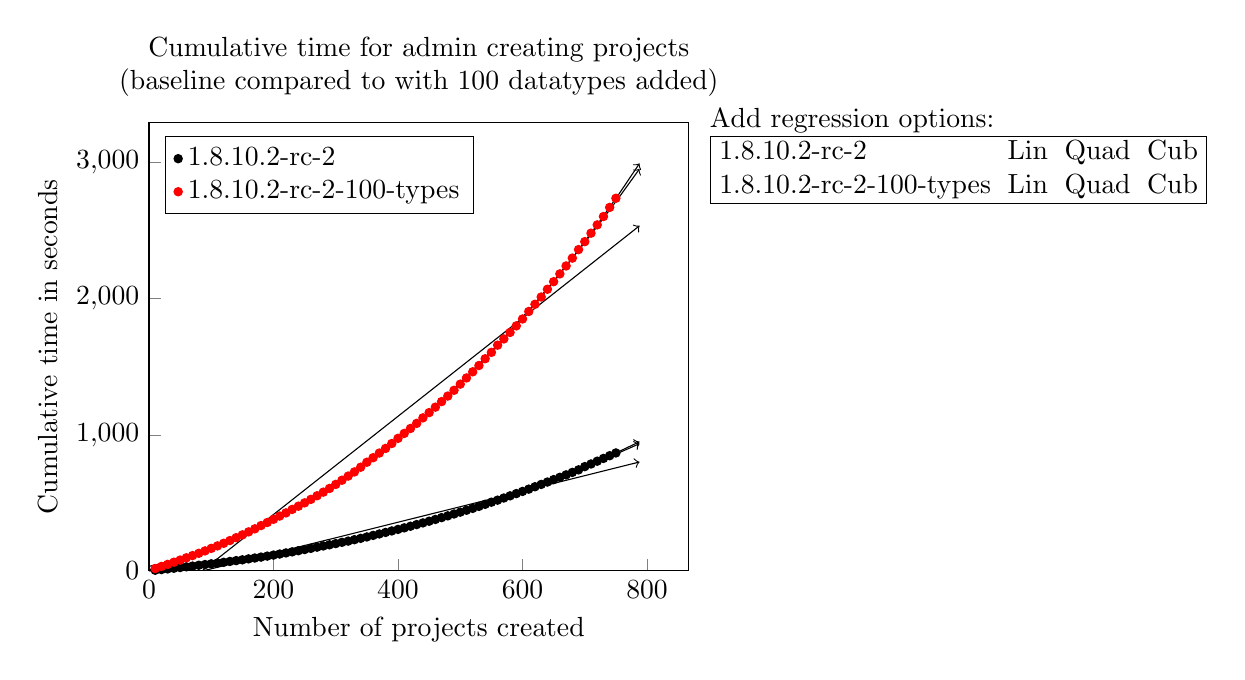
\begin{tikzpicture}
    \begin{axis}[
        align = center,
        legend pos = north west,
        legend cell align = left,
        xlabel = Number of projects created,
        ylabel = Cumulative time in seconds,
        xtick pos = left,
        ytick pos = left,
        scaled ticks = false,
        xmin = 0,
        ymin = 0,
        title = {Cumulative time for admin creating projects (baseline compared to with 100 datatypes added)},
        title style = {text width = 0.8\textwidth},
        legend entries={\switchocg{1.8.10.2-rc-2}{1.8.10.2-rc-2},\switchocg{1.8.10.2-rc-2-100-types}{1.8.10.2-rc-2-100-types}}]
        \begin{scope}[ocg = {ref = 1.8.10.2-rc-2-Lin, status = invisible}]
            \plot[domain=0:788,->,forget plot] (\x,{-98.5433167567568517597464960999786853790283203125 + 1.1410233598862020709674425233970396220684051513671875*(\x)^1});
        \end{scope}
        \begin{scope}[ocg = {ref = 1.8.10.2-rc-2-Quad, status = invisible}]
            \plot[domain=0:788,->,forget plot] (\x,{11.1593722473155256835752879851497709751129150390625 + 0.28619721180252055692250223728478886187076568603515625*(\x)^1 + 0.0011247712474785286594636257717638727626763284206390380859375*(\x)^2});
        \end{scope}
        \begin{scope}[ocg = {ref = 1.8.10.2-rc-2-Cub, status = invisible}]
            \plot[domain=0:788,->,forget plot] (\x,{1.27564702949494357397952626342885196208953857421875 + 0.437275798982397656544662822852842509746551513671875*(\x)^1 + 0.00063107867915582010163999537866175160161219537258148193359375*(\x)^2 + 0.00000043306365642342866221573276404310792742080593598075211048126220703125*(\x)^3});
        \end{scope}
        \begin{scope}[ocg = {ref = 1.8.10.2-rc-2, status = visible}]
            \addplot[
                only marks,
                color = black,
                mark = *,
                mark size = 1.5 pt
            ]coordinates {(10,5.155)(20,10.073)(30,14.993)(40,19.829)(50,24.93)(60,30.281)(70,35.564)(80,41.778)(90,47.008)(100,52.396)(110,57.855)(120,63.463)(130,69.754)(140,75.835)(150,81.721)(160,88.623)(170,94.963)(180,101.755)(190,109.012)(200,116.5)(210,124.353)(220,132.284)(230,140.113)(240,148.531)(250,157.21)(260,165.941)(270,174.78)(280,183.646)(290,192.075)(300,200.944)(310,210.274)(320,219.287)(330,229.541)(340,239.692)(350,249.866)(360,261.059)(370,271.873)(380,282.988)(390,293.951)(400,305.193)(410,316.567)(420,328.482)(430,340.614)(440,352.935)(450,365.329)(460,378.286)(470,391.663)(480,404.815)(490,418.442)(500,431.939)(510,445.962)(520,459.688)(530,474.24)(540,489.597)(550,505.032)(560,520.093)(570,535.912)(580,551.828)(590,568.228)(600,584.308)(610,601.015)(620,618.633)(630,635.712)(640,653.223)(650,670.959)(660,688.079)(670,705.978)(680,724.029)(690,742.705)(700,766.442)(710,785.774)(720,806.436)(730,826.67)(740,846.753)(750,866.96)};
        \end{scope}
        \begin{scope}[ocg = {ref = 1.8.10.2-rc-2-100-types-Lin, status = invisible}]
            \plot[domain=0:788,->,forget plot] (\x,{-307.29821909909827581941499374806880950927734375 + 3.608704716927451983110586297698318958282470703125*(\x)^1});
        \end{scope}
        \begin{scope}[ocg = {ref = 1.8.10.2-rc-2-100-types-Quad, status = invisible}]
            \plot[domain=0:788,->,forget plot] (\x,{33.5855459755653811271258746273815631866455078125 + 0.9524675864755269838468620946514420211315155029296875*(\x)^1 + 0.00349504885585779669077144404809587285853922367095947265625*(\x)^2});
        \end{scope}
        \begin{scope}[ocg = {ref = 1.8.10.2-rc-2-100-types-Cub, status = invisible}]
            \plot[domain=0:788,->,forget plot] (\x,{6.12879746842850980925732073956169188022613525390625 + 1.3721602308574525341811067846720106899738311767578125*(\x)^1 + 0.0021235828964603427511381728010064762202091515064239501953125*(\x)^2 + 0.0000012030403152609250939431874416474244071650900878012180328369140625*(\x)^3});
        \end{scope}
        \begin{scope}[ocg = {ref = 1.8.10.2-rc-2-100-types, status = visible}]
            \addplot[
                only marks,
                color = red,
                mark = *,
                mark size = 1.5 pt
            ]coordinates {(10,17.813)(20,33.07)(30,48.279)(40,64.101)(50,79.811)(60,96.463)(70,112.821)(80,129.532)(90,147.275)(100,165.84)(110,184.021)(120,203.426)(130,223.257)(140,244.118)(150,265.029)(160,287.091)(170,309.455)(180,333.482)(190,355.978)(200,379.523)(210,403.448)(220,426.406)(230,451.938)(240,475.801)(250,500.26)(260,525.828)(270,552.49)(280,579.029)(290,606.123)(300,635.944)(310,666.698)(320,697.255)(330,727.638)(340,762.153)(350,798.695)(360,832.01)(370,866.252)(380,900.303)(390,936.293)(400,974.143)(410,1010.42)(420,1046.868)(430,1084.382)(440,1124.774)(450,1163.351)(460,1203.521)(470,1244.204)(480,1285.033)(490,1327.322)(500,1372.484)(510,1418.032)(520,1463.178)(530,1509.456)(540,1559.258)(550,1606.108)(560,1658.98)(570,1704.807)(580,1752.348)(590,1800.751)(600,1851.268)(610,1906.337)(620,1959.516)(630,2012.801)(640,2069.765)(650,2125.403)(660,2182.744)(670,2240.983)(680,2298.568)(690,2361.177)(700,2419.57)(710,2481.858)(720,2542.768)(730,2604.069)(740,2671.131)(750,2738.391)};
        \end{scope}
    \end{axis}
    \begin{scope}
        \addtolength{\tabcolsep}{-0.3em}
        \node [below right, shape=rectangle, align=left](regressiontable) at (7,6) {
            Add regression options: \\
            \begin{tabular}{|llll|}
                \hline
                1.8.10.2-rc-2 & \switchocg{1.8.10.2-rc-2-Lin}{Lin} & \switchocg{1.8.10.2-rc-2-Quad}{Quad} & \switchocg{1.8.10.2-rc-2-Cub}{Cub} \\
                1.8.10.2-rc-2-100-types & \switchocg{1.8.10.2-rc-2-100-types-Lin}{Lin} & \switchocg{1.8.10.2-rc-2-100-types-Quad}{Quad} & \switchocg{1.8.10.2-rc-2-100-types-Cub}{Cub} \\
                \hline
            \end{tabular}
        };
    \end{scope}
\end{tikzpicture}

\end{document}